\begin{figure}[ht]
	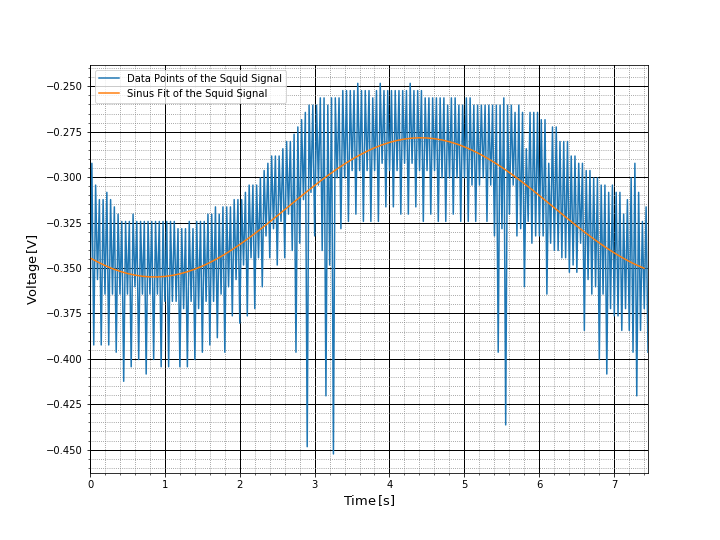
\includegraphics[scale=0.5]{Bild/r1_5_1}
	\centering
	\caption[Plot of first conductor loop 1]{Plot 1 of the first conductor loop with resistor R1. The speed of the rotation here was 5. In orange is the sinus fit of the data point.}
\end{figure}
\begin{figure}[ht]
	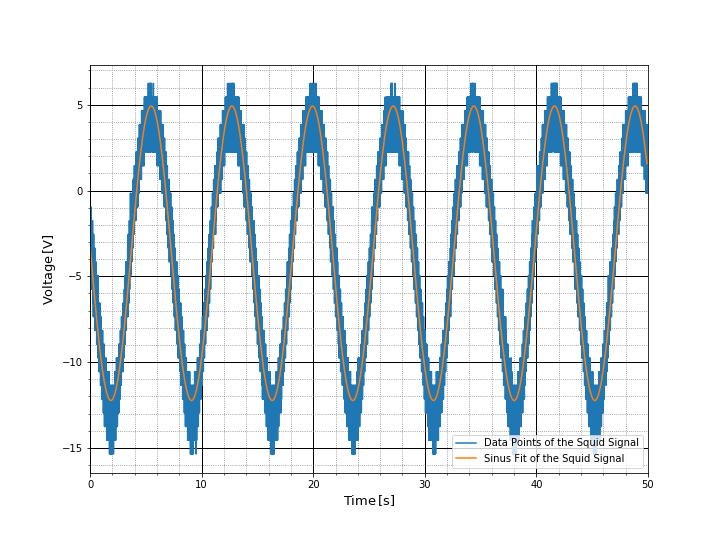
\includegraphics[scale=0.5]{Bild/r1_5_2}
	\centering
	\caption[Plot of first conductor loop 2 ]{Plot 2 of the first conductor loop with resistor R1. The speed of the rotation here was 5. In orange is the sinus fit of the data point.}
\end{figure}
\begin{figure}[ht]
	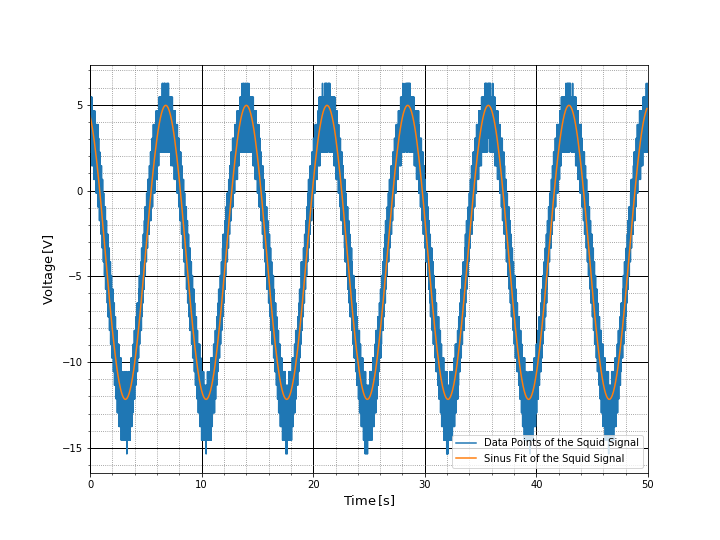
\includegraphics[scale=0.5]{Bild/r1_5_3}
	\centering
	\caption[Plot of first conductor loop 3]{Plot 3 of the first conductor loop with resistor R1. The speed of the rotation here was 5. In orange is the sinus fit of the data point.}
\end{figure}
\begin{figure}[ht]
	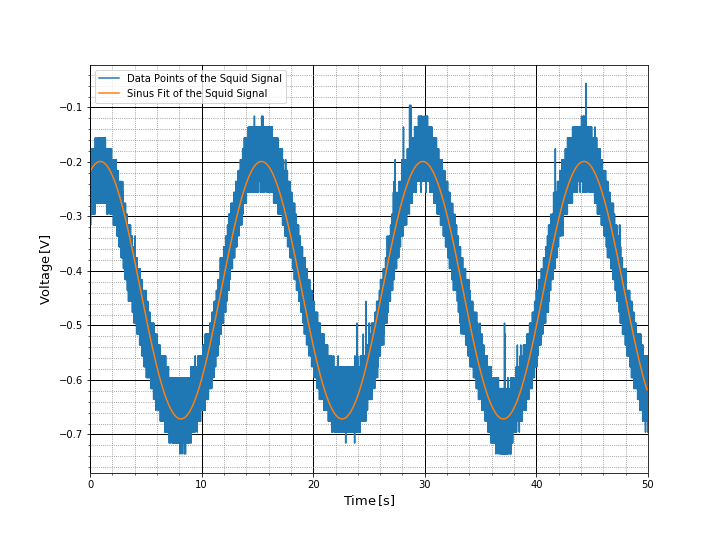
\includegraphics[scale=0.5]{Bild/r1_5_4}
	\centering
	\caption[Plot of first conductor loop 4]{Plot 4 of the first conductor loop with resistor R1. The speed of the rotation here was 5. In orange is the sinus fit of the data point.}
\end{figure}
\begin{figure}[ht]
	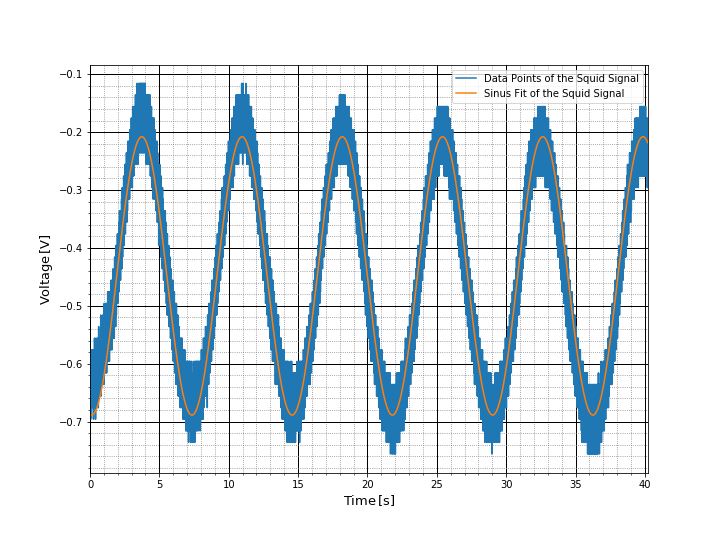
\includegraphics[scale=0.5]{Bild/r1_10_1}
	\centering
	\caption[Plot of first conductor loop 5]{Plot 5 of the first conductor loop with resistor R1. The speed of the rotation here was 10. In orange is the sinus fit of the data point.}
\end{figure}
\begin{figure}[ht]
	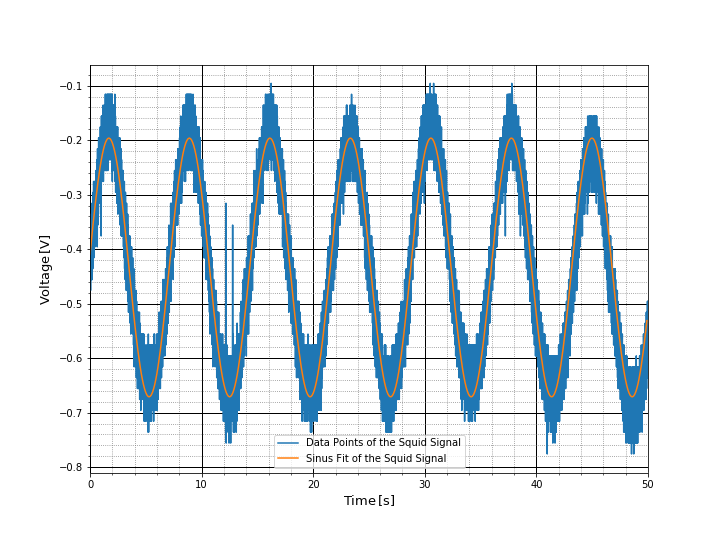
\includegraphics[scale=0.5]{Bild/r1_10_2}
	\centering
	\caption[Plot of first conductor loop 6]{Plot 6 of the first conductor loop with resistor R1. The speed of the rotation here was 10. In orange is the sinus fit of the data point.}
\end{figure}
\begin{figure}[ht]
	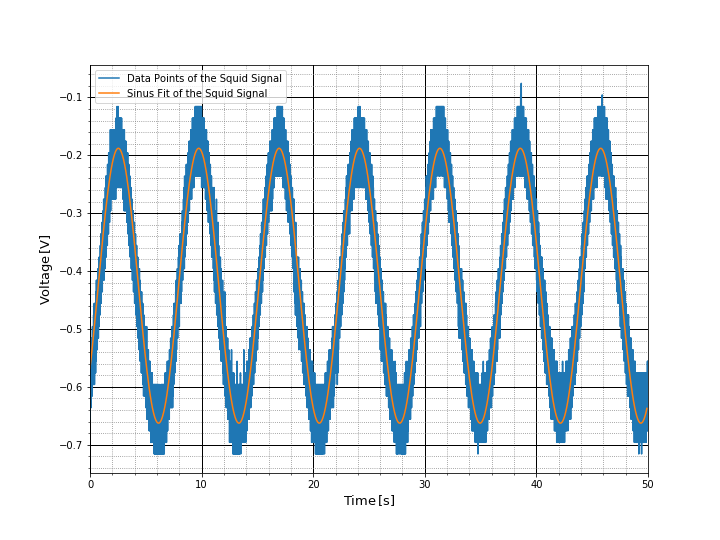
\includegraphics[scale=0.5]{Bild/r1_10_3}
	\centering
	\caption[Plot of first conductor loop 7]{Plot 7 of the first conductor loop with resistor R1. The speed of the rotation here was 10. In orange is the sinus fit of the data point.}
\end{figure}
\begin{figure}[ht]
	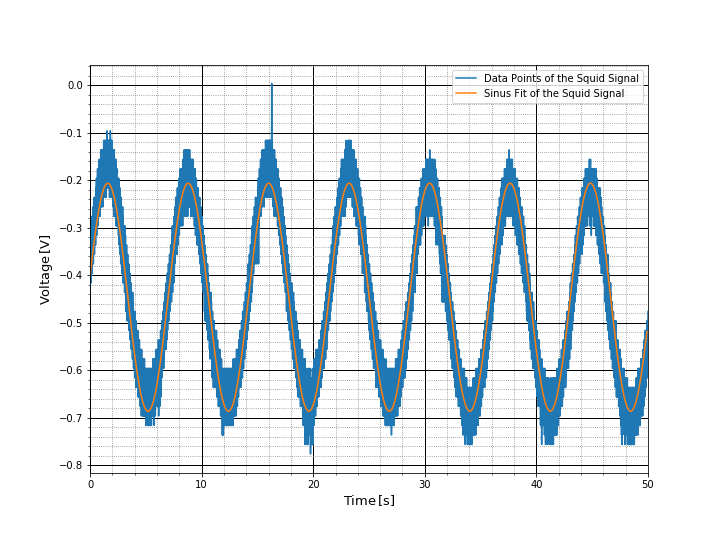
\includegraphics[scale=0.5]{Bild/r1_10_4}
	\centering
	\caption[Plot of first conductor loop 8]{Plot 8 of the first conductor loop with resistor R1. The speed of the rotation here was 10. In orange is the sinus fit of the data point.}
\end{figure}
\begin{figure}[ht]
	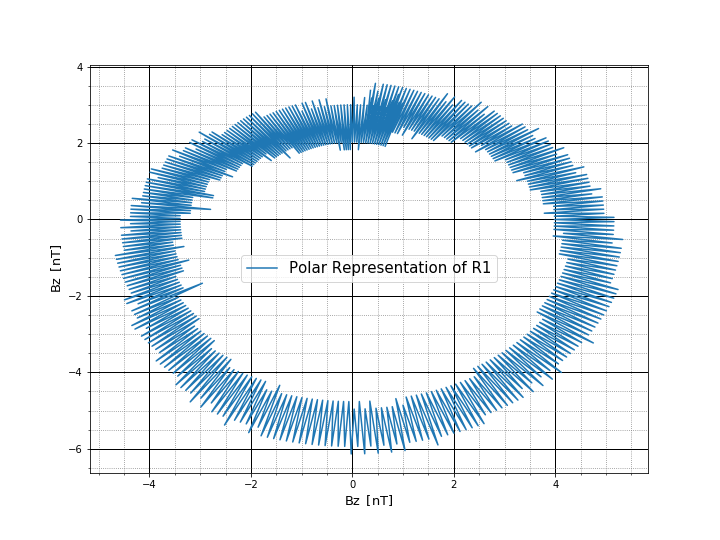
\includegraphics[scale=0.5]{Bild/R1}
	\centering
	\caption[Polar Representation for R1 Conductor Loop]{Polar Representation for one period of the signal coming from the R1 Conductor Loop.}
\end{figure}
\begin{figure}[ht]
	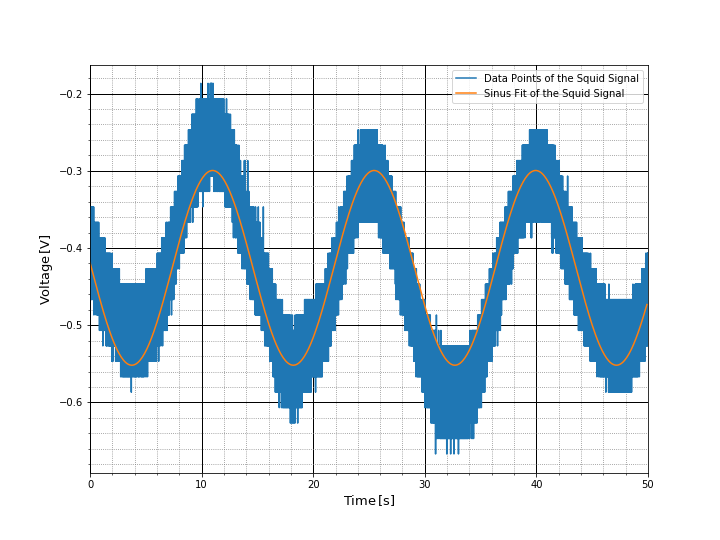
\includegraphics[scale=0.5]{Bild/r2_5_1}
	\centering
	\caption[Plot of second conductor loop 1]{Plot 1 of the second conductor loop with resistor 2. The speed of the rotation here was 5. In orange is the sinus fit of the data point.}
\end{figure}
\begin{figure}[ht]
	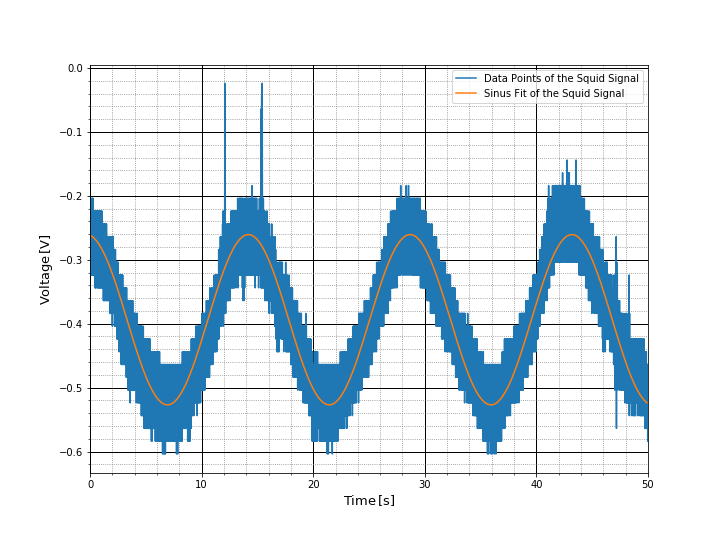
\includegraphics[scale=0.5]{Bild/r2_5_2}
	\centering
	\caption[Plot of second conductor loop 2]{Plot 2 of the second conductor loop with resistor 2. The speed of the rotation here was 5. In orange is the sinus fit of the data point.}
\end{figure}
\begin{figure}[ht]
	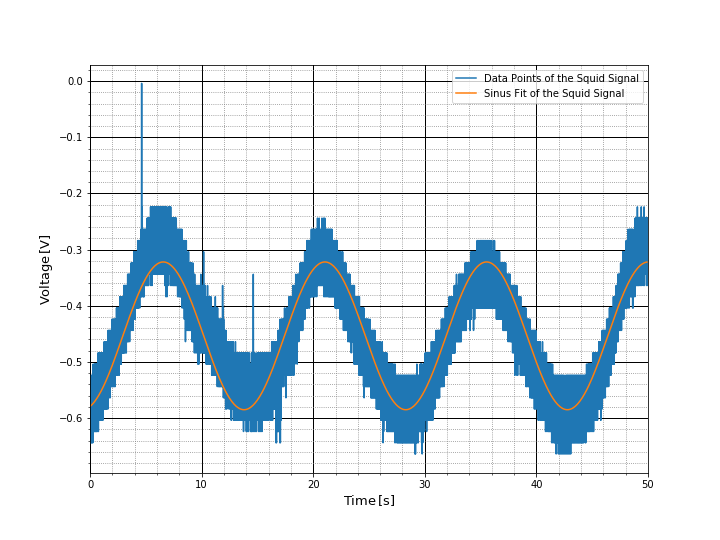
\includegraphics[scale=0.5]{Bild/r2_5_3}
	\centering
	\caption[Plot of second conductor loop 3]{Plot 3 of the second conductor loop with resistor 2. The speed of the rotation here was 5. In orange is the sinus fit of the data point.}
\end{figure}
\begin{figure}[ht]
	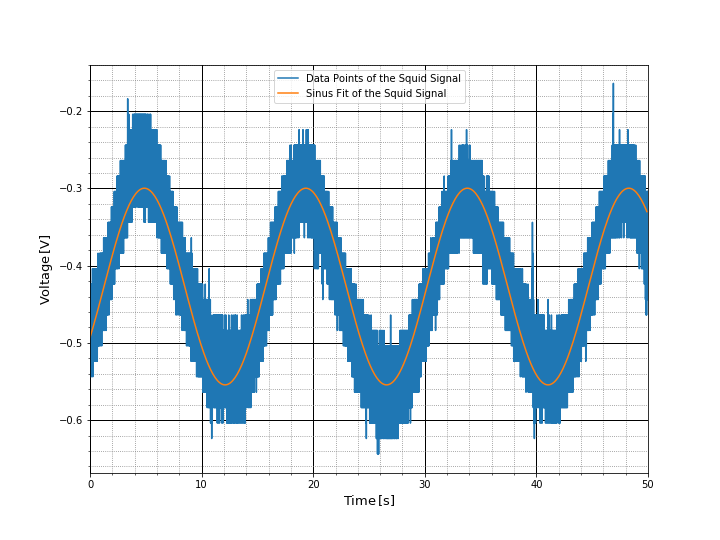
\includegraphics[scale=0.5]{Bild/r2_5_4}
	\centering
	\caption[Plot of second conductor loop 4]{Plot 4 of the second conductor loop with resistor 2. The speed of the rotation here was 5. In orange is the sinus fit of the data point.}
\end{figure}
\begin{figure}[ht]
	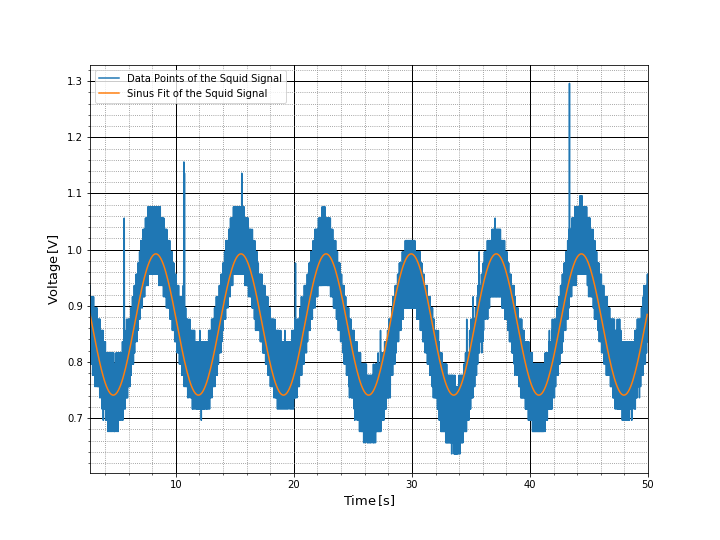
\includegraphics[scale=0.5]{Bild/r2_10_1}
	\centering
	\caption[Plot of second conductor loop 5]{Plot 5 of the second conductor loop with resistor 2. The speed of the rotation here was 10. In orange is the sinus fit of the data point.}
\end{figure}
\begin{figure}[ht]
	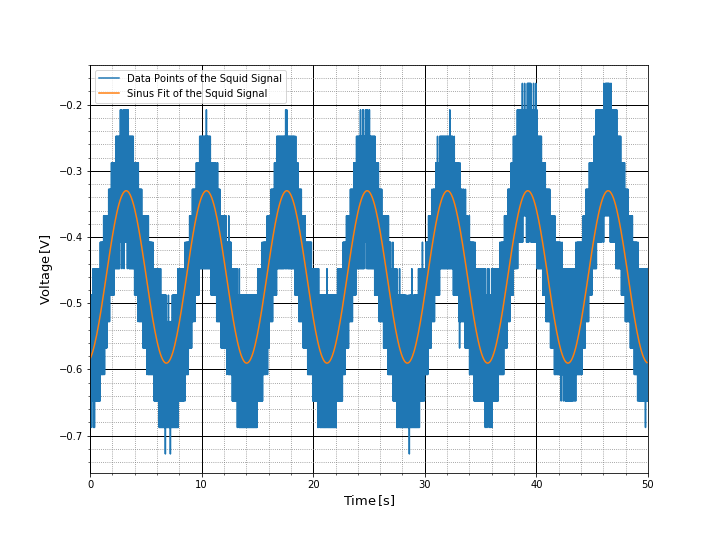
\includegraphics[scale=0.5]{Bild/r2_10_2}
	\centering
	\caption[Plot of second conductor loop 6]{Plot 6 of the second conductor loop with resistor 2. The speed of the rotation here was 10. In orange is the sinus fit of the data point.}
\end{figure}
\begin{figure}[ht]
	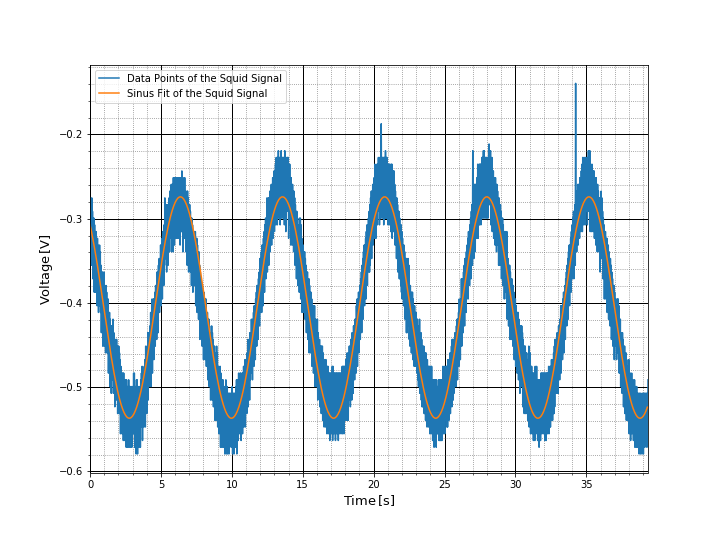
\includegraphics[scale=0.5]{Bild/r2_10_3}
	\centering
	\caption[Plot of second conductor loop 7]{Plot 7 of the second conductor loop with resistor 2. The speed of the rotation here was 10. In orange is the sinus fit of the data point.}
\end{figure}
\begin{figure}[ht]
	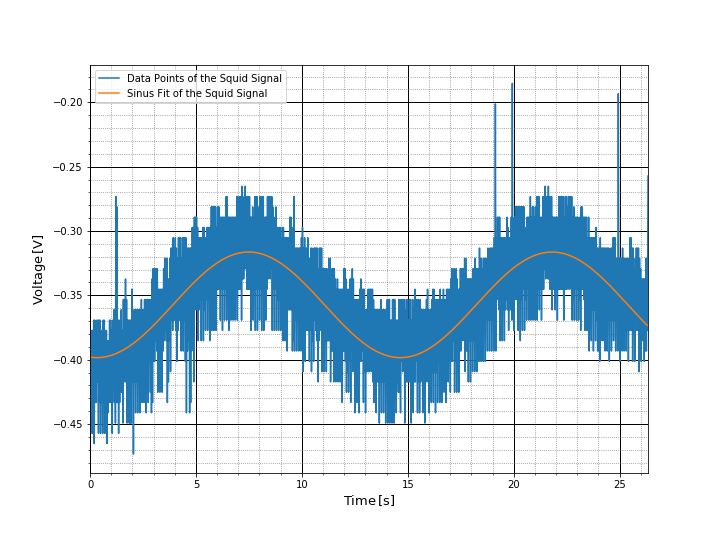
\includegraphics[scale=0.5]{Bild/r3_5_1}
	\centering
	\caption[Plot of third conductor loop 1]{Plot 1 of the third conductor loop with resistor 3. The speed of the rotation here was 5. In orange is the sinus fit of the data point.}
\end{figure}
\begin{figure}[ht]
	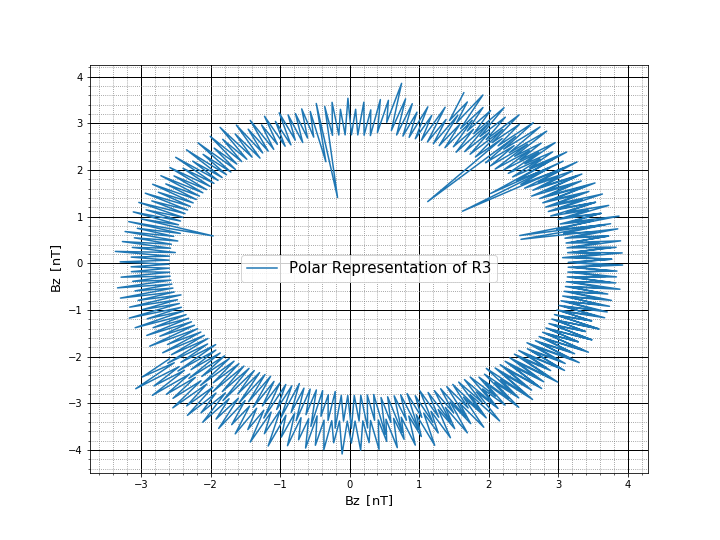
\includegraphics[scale=0.5]{Bild/R3}
	\centering
	\caption[Polar Representation for R3 Conductor Loop]{Polar Representation for one period of the signal coming from the R3 Conductor Loop.}
\end{figure}
\begin{figure}[ht]
	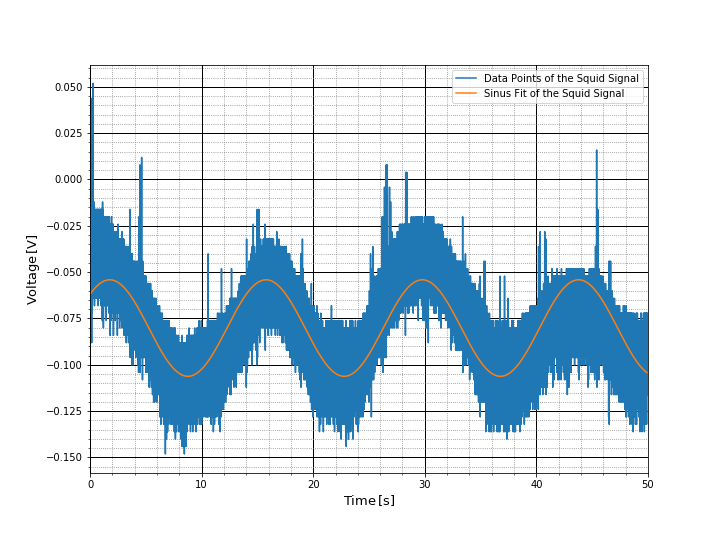
\includegraphics[scale=0.5]{Bild/r4_5_1}
	\centering
	\caption[Plot of fourth conductor loop 1]{Plot 1 of the fourth conductor loop with resistor 4. The speed of the rotation here was 5. In orange is the sinus fit of the data point.}
\end{figure}
\begin{figure}[ht]
	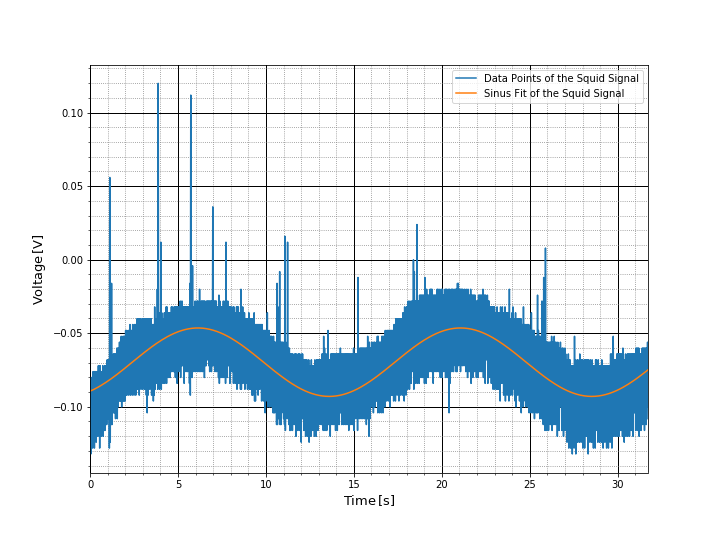
\includegraphics[scale=0.5]{Bild/r4_5_2}
	\centering
	\caption[Plot of fourth conductor loop 2]{Plot 2 of the fourth conductor loop with resistor 4. The speed of the rotation here was 5. In orange is the sinus fit of the data point.}
\end{figure}
\begin{figure}[ht]
	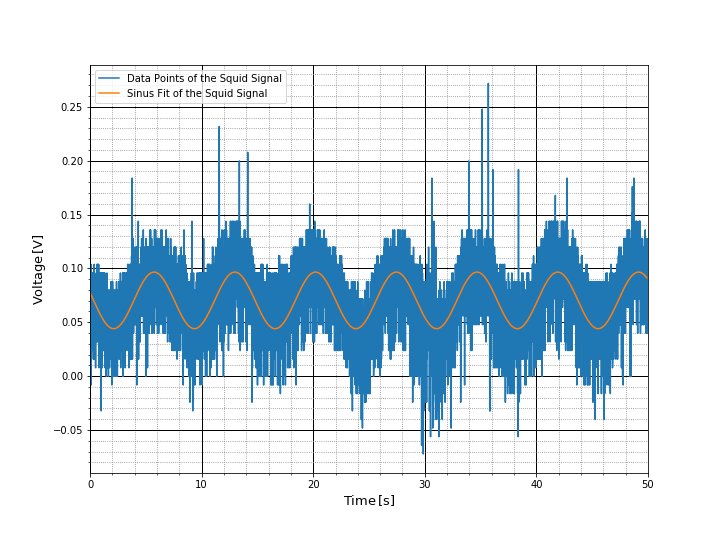
\includegraphics[scale=0.5]{Bild/r4_10_1}
	\centering
	\caption[Plot of fourth conductor loop 3]{Plot 3 of the fourth conductor loop with resistor 4. The speed of the rotation here was 10. In orange is the sinus fit of the data point.}
\end{figure}
\begin{figure}[ht]
	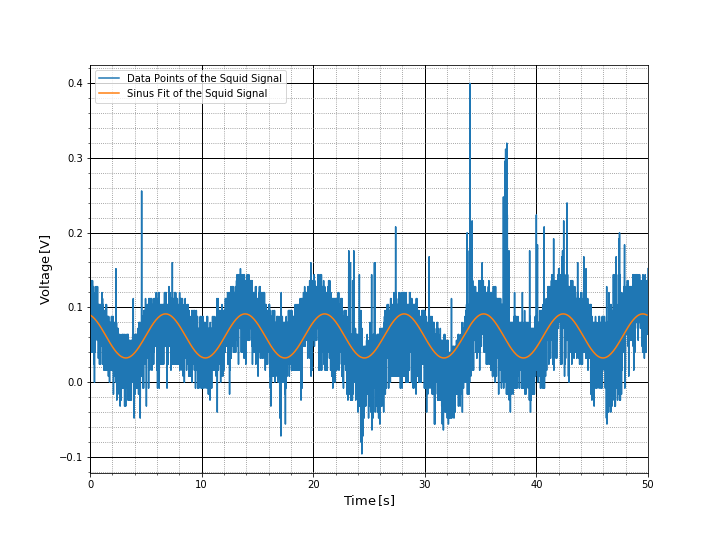
\includegraphics[scale=0.5]{Bild/r4_10_2}
	\centering
	\caption[Plot of fourth conductor loop 4]{Plot 4 of the fourth conductor loop with resistor 4. The speed of the rotation here was 10. In orange is the sinus fit of the data point.}
\end{figure}
\begin{figure}[ht]
	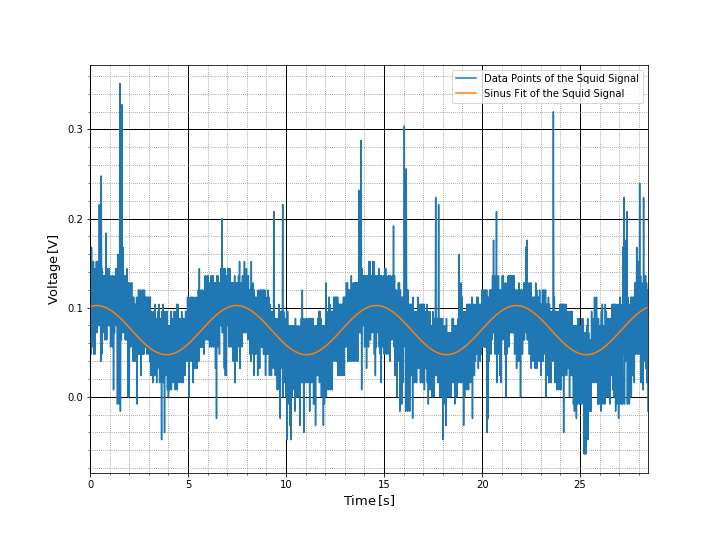
\includegraphics[scale=0.5]{Bild/r4_10_3}
	\centering
	\caption[Plot of fourth conductor loop 5]{Plot 5 of the fourth conductor loop with resistor 4. The speed of the rotation here was 10. In orange is the sinus fit of the data point.}
\end{figure}
\begin{figure}[ht]
	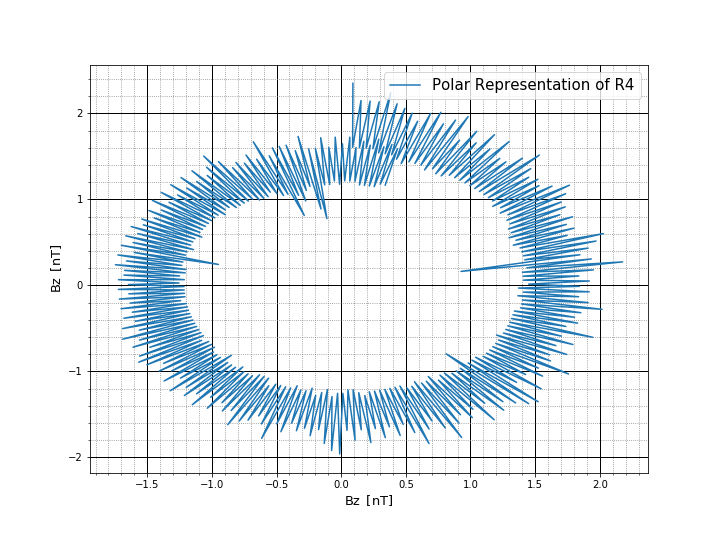
\includegraphics[scale=0.5]{Bild/R4}
	\centering
	\caption[Polar Representation for R4 Conductor Loop]{Polar Representation for one period of the signal coming from the R4 Conductor Loop.}
\end{figure}
\begin{figure}[ht]
	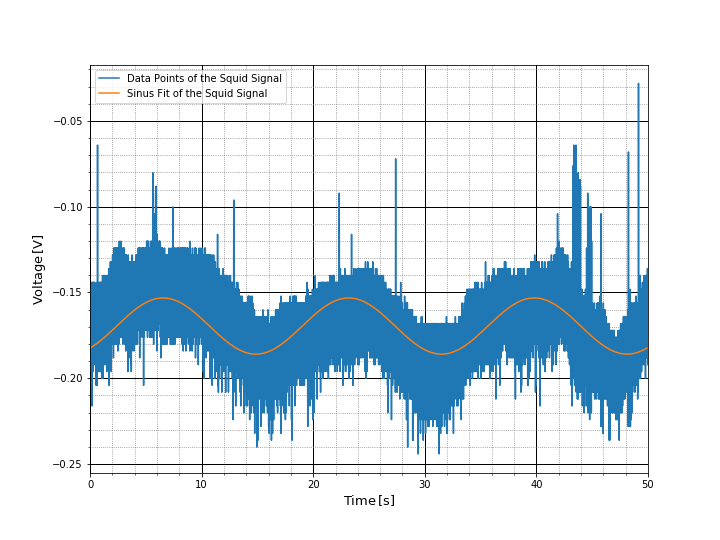
\includegraphics[scale=0.5]{Bild/r5_5_2}
	\centering
	\caption[Plot of fifth conductor loop 1]{Plot 1 of the fifth conductor loop with resistor 5. The speed of the rotation here was 5. In orange is the sinus fit of the data point.}
\end{figure}
\begin{figure}[ht]
	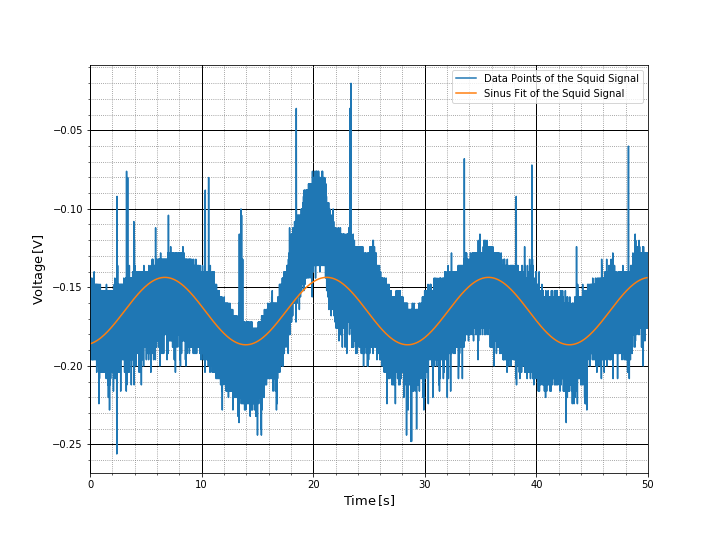
\includegraphics[scale=0.5]{Bild/r5_5_3}
	\centering
	\caption[Plot of fifth conductor loop 2]{Plot 2 of the fifth conductor loop with resistor 5. The speed of the rotation here was 5. In orange is the sinus fit of the data point.}
\end{figure}
\begin{figure}[ht]
	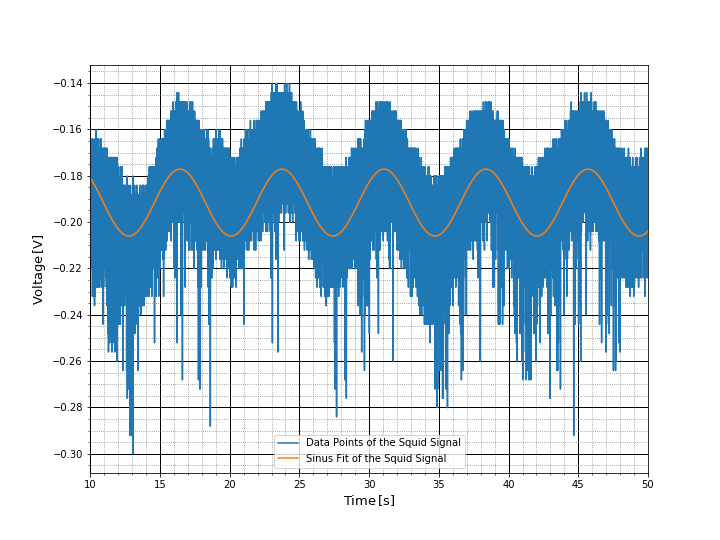
\includegraphics[scale=0.5]{Bild/r5_10_2}
	\centering
	\caption[Plot of fifth conductor loop 3]{Plot 3 of the fifth conductor loop with resistor 5. The speed of the rotation here was 10. In orange is the sinus fit of the data point.}
\end{figure}
\begin{figure}[ht]
	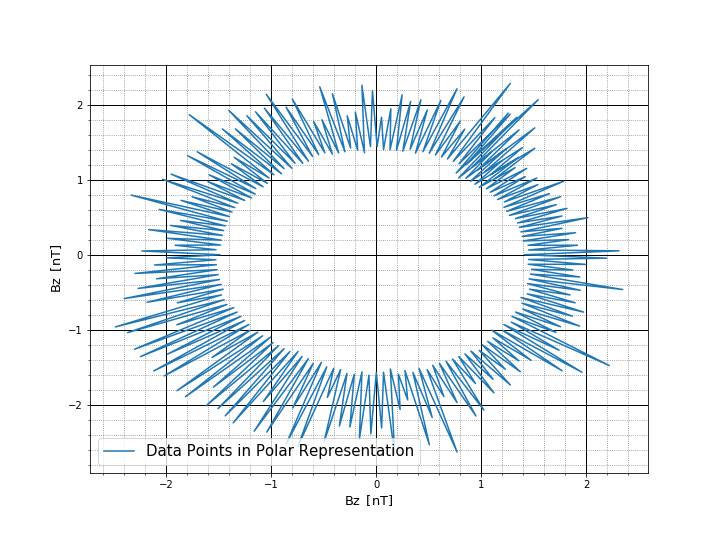
\includegraphics[scale=0.5]{Bild/R5}
	\centering
	\caption[Polar Representation for R5 Conductor Loop]{Polar Representation for one period of the signal coming from the R5 Conductor Loop.}
\end{figure}
\begin{figure}[ht]
	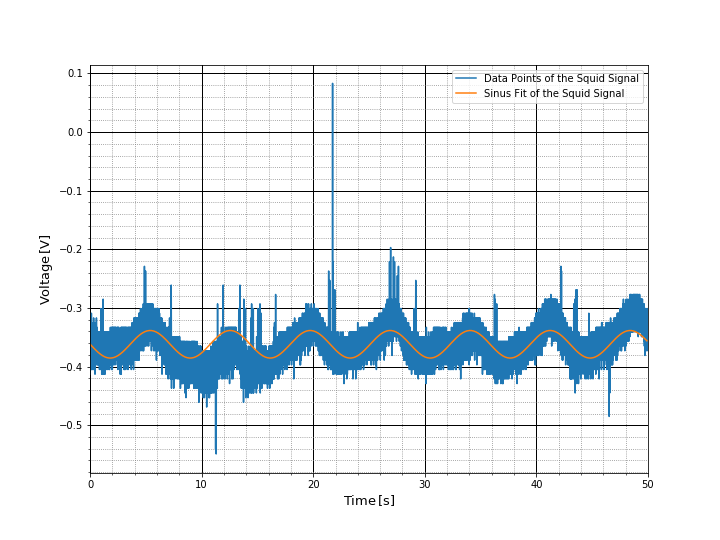
\includegraphics[scale=0.5]{Bild/P1_1}
	\centering
	\caption[SQUID signal of Iron Chips 1]{Plot of the SQUID signal with Iron chips as a sample.}
\end{figure}
\begin{figure}[ht]
	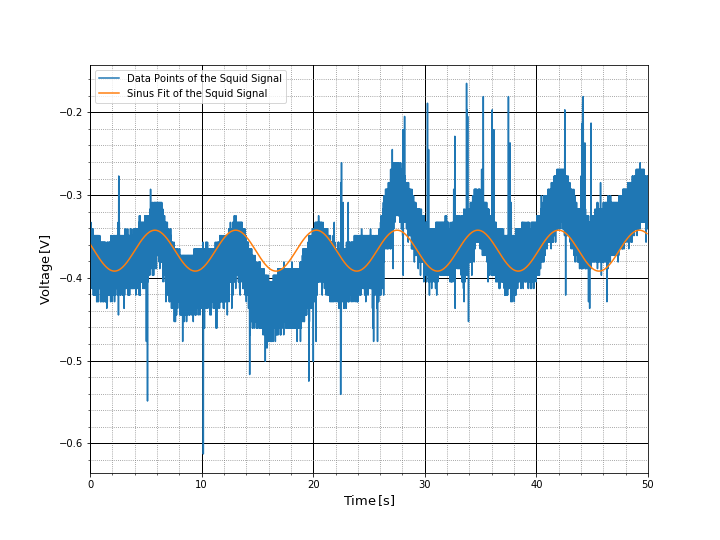
\includegraphics[scale=0.5]{Bild/P1_2}
	\centering
	\caption[SQUID signal of Iron Chips 2]{Plot of the SQUID signal with Iron chips as a sample.}
\end{figure}
\begin{figure}[ht]
	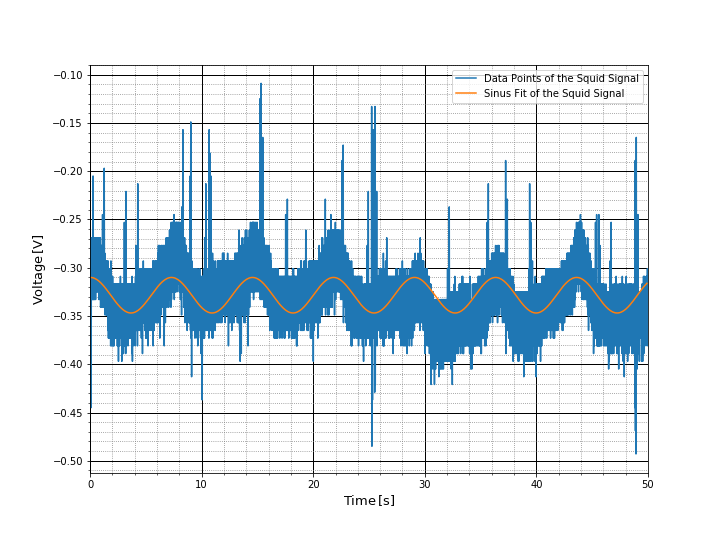
\includegraphics[scale=0.5]{Bild/P1_3}
	\centering
	\caption[SQUID signal of Iron Chips 3]{Plot of the SQUID signal with Iron chips as a sample.}
\end{figure}
\begin{figure}[ht]
	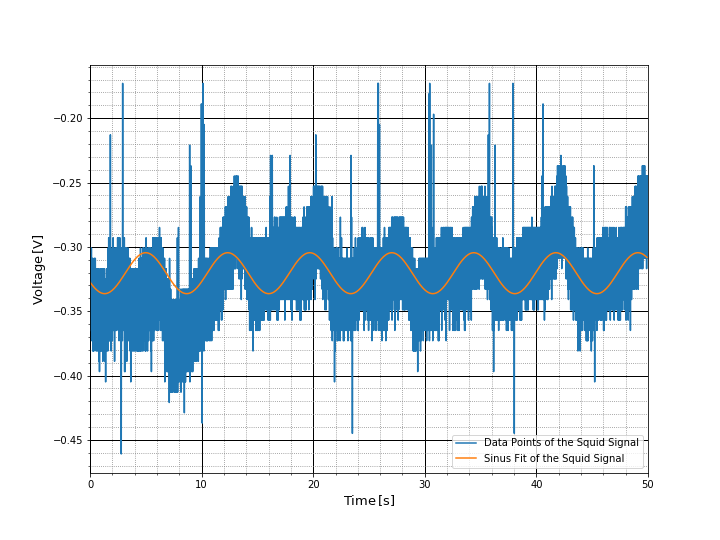
\includegraphics[scale=0.5]{Bild/P1_4}
	\centering
	\caption[SQUID signal of Iron Chips 4]{Plot of the SQUID signal with Iron chips as a sample.}
\end{figure}
\begin{figure}[ht]
	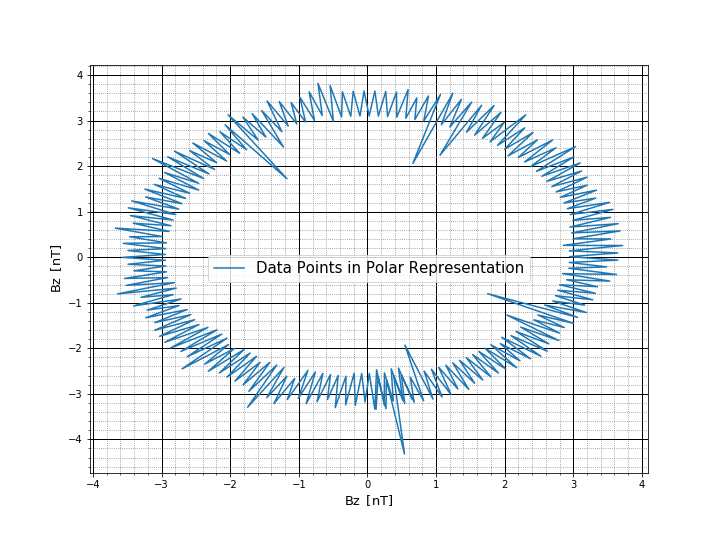
\includegraphics[scale=0.5]{Bild/Eisenstaub}
	\centering
	\caption[Polar Representation for Iron Chips]{Polar Representation for one period of the signal coming from the iron chips.}
\end{figure}
\begin{figure}[ht]
	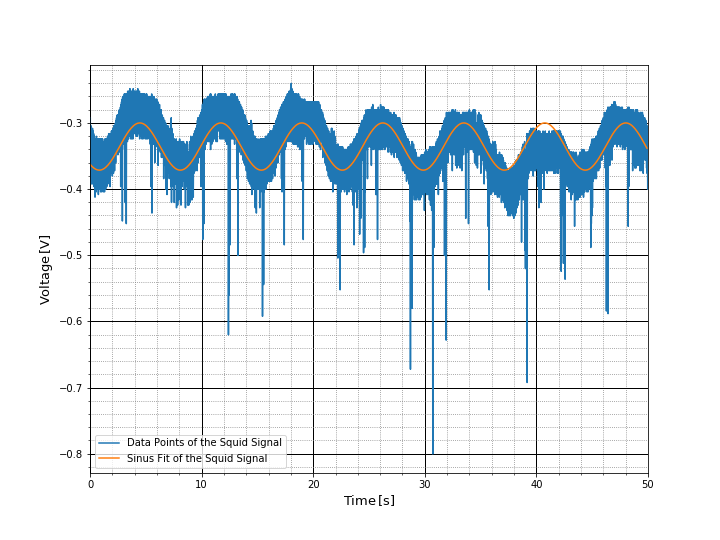
\includegraphics[scale=0.5]{Bild/P2_1}
	\centering
	\caption[SQUID signal of a Gold Slide 1]{Plot of the SQUID signal with Gold Slide as a sample.}
\end{figure}
\begin{figure}[ht]
	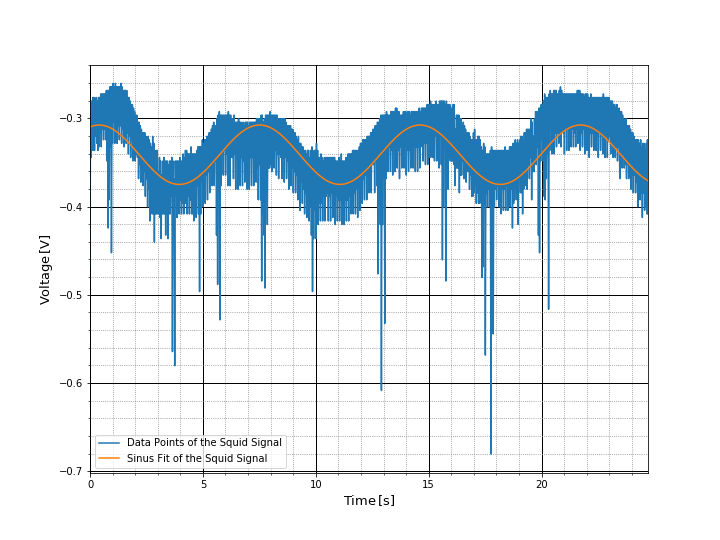
\includegraphics[scale=0.5]{Bild/P2_2}
	\centering
	\caption[SQUID signal of a Gold Slide 2]{Plot of the SQUID signal with Gold Slide as a sample.}
\end{figure}
\begin{figure}[ht]
	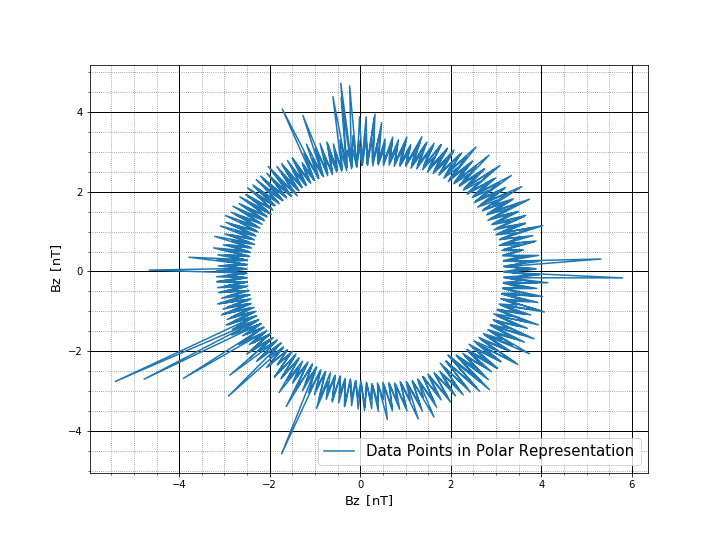
\includegraphics[scale=0.5]{Bild/Gold}
	\centering
	\caption[Polar Representation for Gold Slide]{Polar Representation for one period of the signal coming from the gold slide.}
\end{figure}
\begin{figure}[ht]
	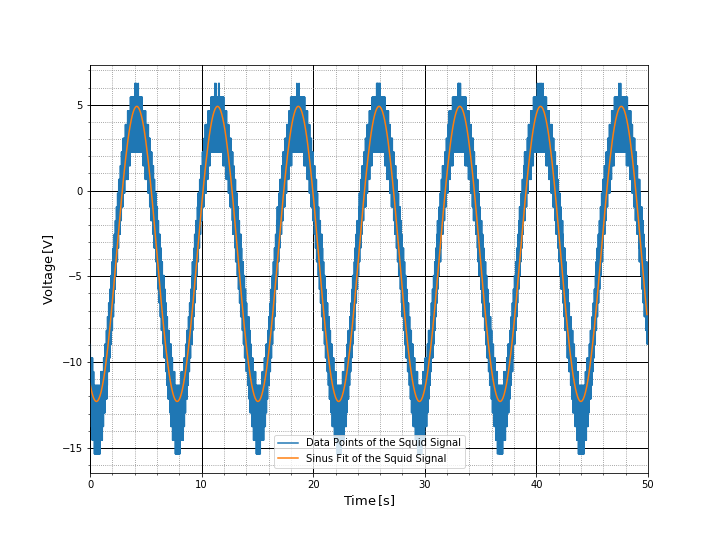
\includegraphics[scale=0.5]{Bild/P3_1}
	\centering
	\caption[SQUID signal of Magnet Chips 1]{Plot of the SQUID signal with Magnet chips as a sample.}
\end{figure}
\begin{figure}[ht]
	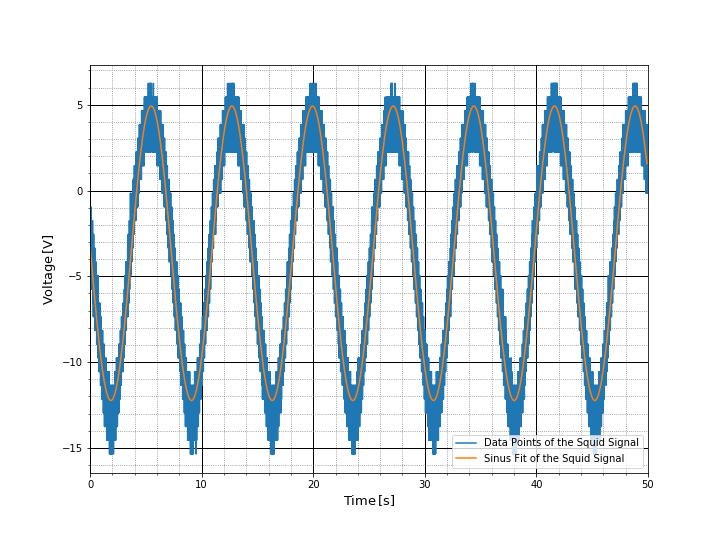
\includegraphics[scale=0.5]{Bild/P3_2}
	\centering
	\caption[SQUID signal of Magnet Chips 2]{Plot of the SQUID signal with Magnet chips as a sample.}
\end{figure}
\begin{figure}[ht]
	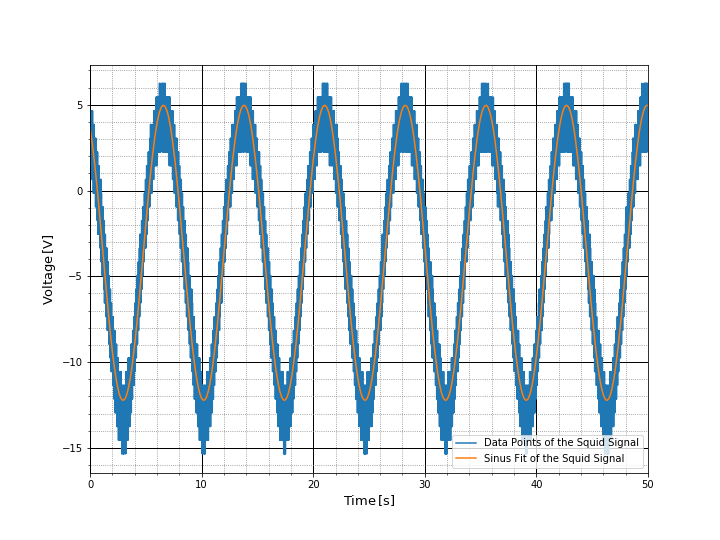
\includegraphics[scale=0.5]{Bild/P3_3}
	\centering
	\caption[SQUID signal of Magnet Chips 3]{Plot of the SQUID signal with Magnet chips as a sample.}
\end{figure}
\begin{figure}[ht]
	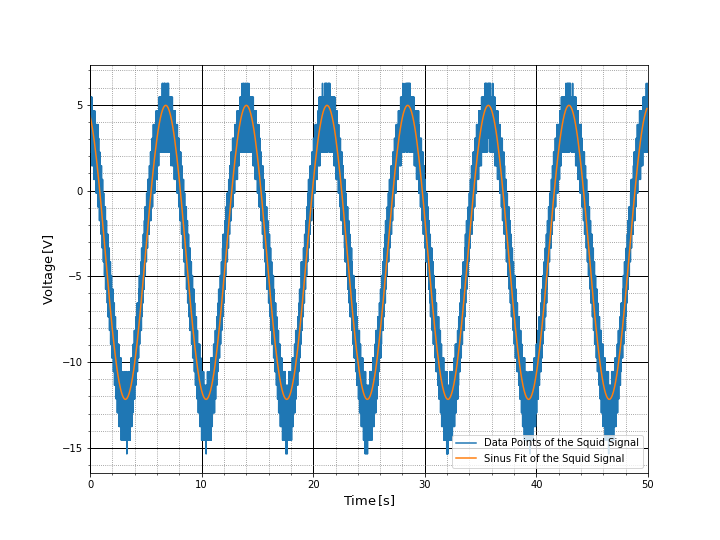
\includegraphics[scale=0.5]{Bild/P3_4}
	\centering
	\caption[SQUID signal of Magnet Chips 4]{Plot of the SQUID signal with Magnet chips as a sample.}
\end{figure}
\begin{figure}[ht]
	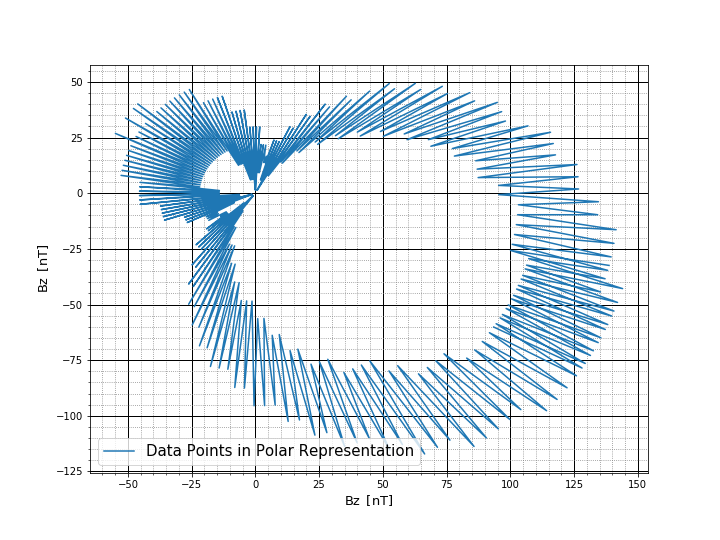
\includegraphics[scale=0.5]{Bild/Magnetspan}
	\centering
	\caption[Polar Representation for Magnet Chips]{Polar Representation for one period of the signal coming from the magnet chips.}
\end{figure}
\begin{figure}[ht]
	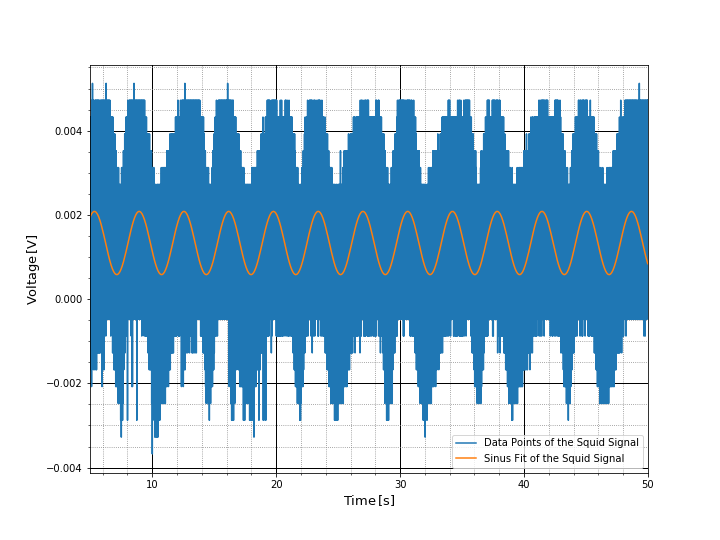
\includegraphics[scale=0.5]{Bild/P4_1}
	\centering
	\caption[SQUID signal of a Stone 1]{Plot of the SQUID signal with a stone as a sample.}
\end{figure}
\begin{figure}[ht]
	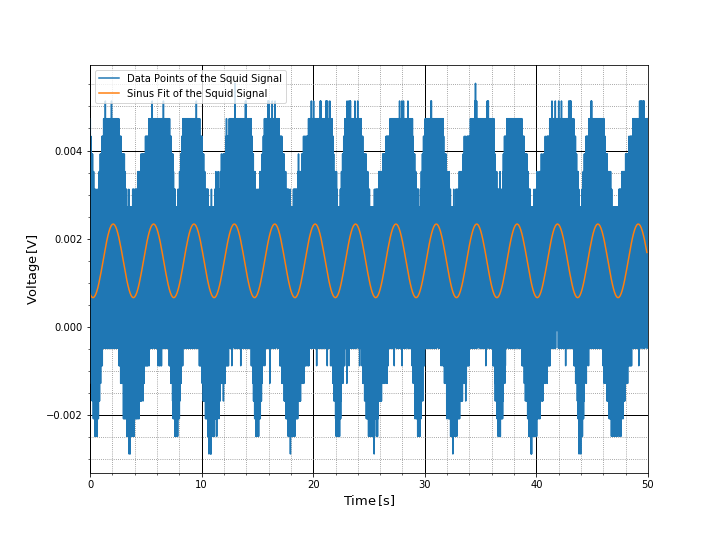
\includegraphics[scale=0.5]{Bild/P4_2}
	\centering
	\caption[SQUID signal of a Stone 2]{Plot of the SQUID signal with a stone as a sample.}
\end{figure}
\begin{figure}[ht]
	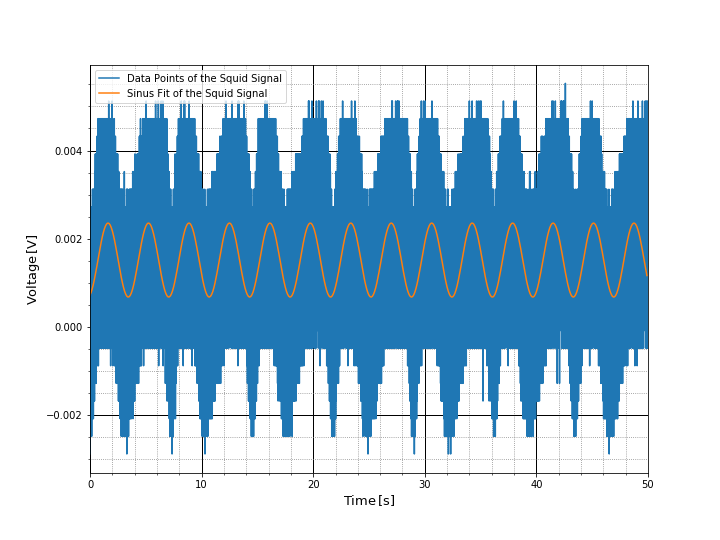
\includegraphics[scale=0.5]{Bild/P4_3}
	\centering
	\caption[SQUID signal of a Stone 3]{Plot of the SQUID signal with a stone as a sample.}
\end{figure}
\begin{figure}[ht]
	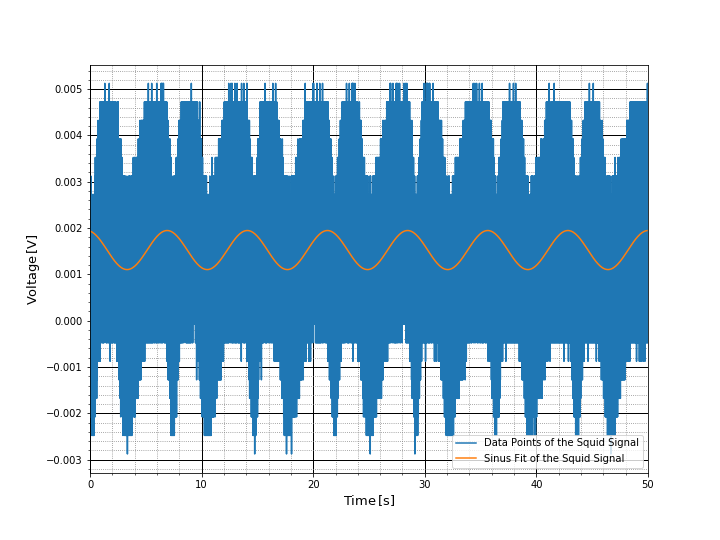
\includegraphics[scale=0.5]{Bild/P4_4}
	\centering
	\caption[SQUID signal of Stone 4]{Plot of the SQUID signal with a Stone as a sample.}
	\ref{Sto}
\end{figure}
\begin{figure}[ht]
	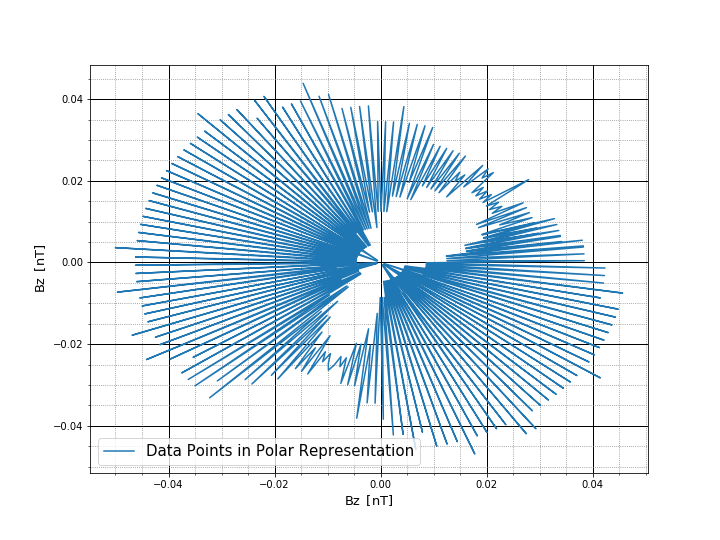
\includegraphics[scale=0.5]{Bild/Stein}
	\centering
	\caption[Polar Representation for a Stone]{Polar Representation for one period of the signal coming from the stone.}
\end{figure}
\begin{figure}[ht]
	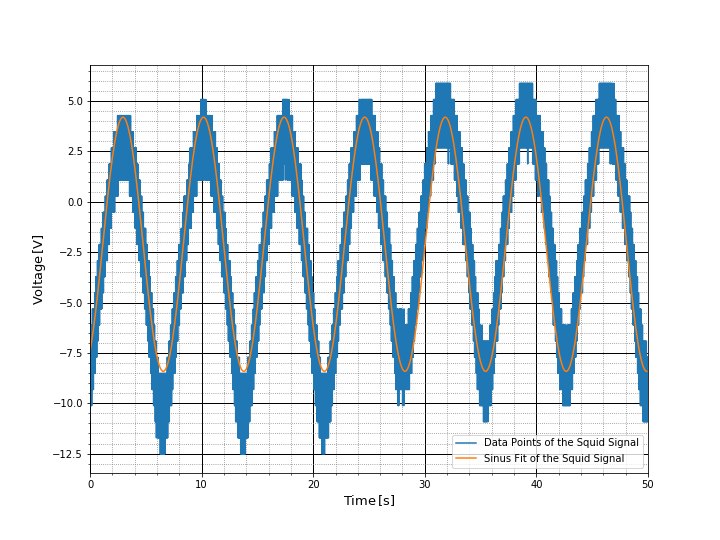
\includegraphics[scale=0.5]{Bild/P5_2}
	\centering
	\caption[SQUID signal of a Magnet 1]{Plot of the SQUID signal with a magnet as a sample.}
\end{figure}
\begin{figure}[ht]
	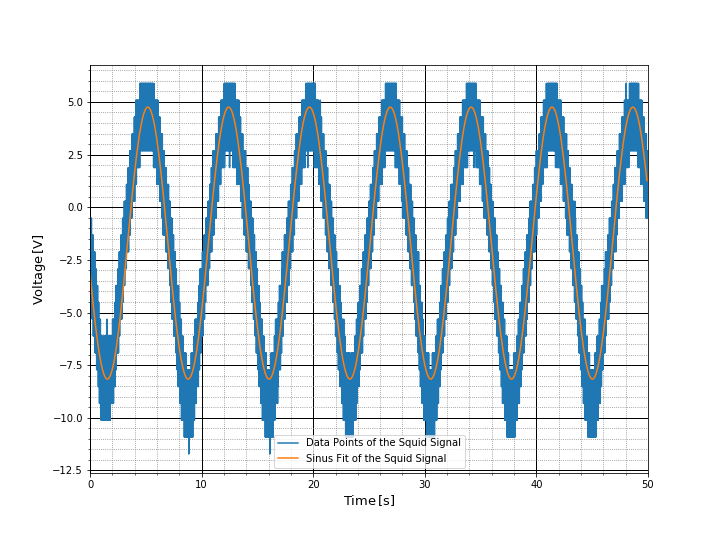
\includegraphics[scale=0.5]{Bild/P5_3}
	\centering
	\caption[SQUID signal of a Magnet 2]{Plot of the SQUID signal with a magnet as a sample.}
\end{figure}
\begin{figure}[ht]
	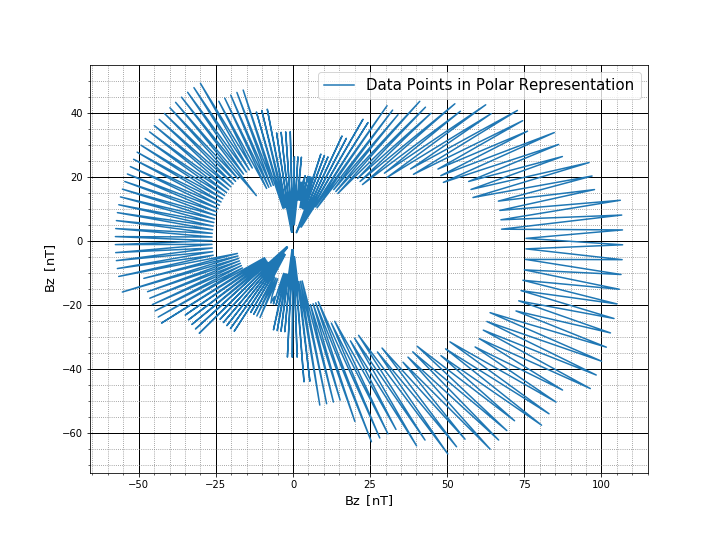
\includegraphics[scale=0.5]{Bild/Magnet}
	\centering
	\caption[Polar Representation for a Magnet]{Polar Representation for one period of the signal coming from the magnet.}
\end{figure}